\chapter{Capitolo 4: Algoritmi basati sulla distanza}
In questo capitolo vengono illustrati i principali algoritmi utilizzati per la costruzione degli alberi evolutivi senza radice. L'obiettivo è quello di trovare una soluzione al cosiddetto \textit{problema degli alberi basati sulla distanza}, ma prima di ciò è necessario introdurre alcuni concetti, tra cui la matrice delle distanze.

\section{Matrice delle distanze}
Dati due punti, $x$ e $y$, la \textit{distanza} può essere vista come loro "lontananza" in uno spazio $k$-dimensionale. Nella fattispecie, è una funzione $d(x,y)$ che possiede le seguenti proprietà \cite{molaCagliari}:
\begin{enumerate}
	\item \textit{non negatività}:
	\[d(x,y)\geq 0\hspace{2em} \forall \: x,y\in R^k\]
	\item \textit{identità}:
	\[d(x,y)=0 \; \leftrightarrow \; x=y\]
	\item \textit{simmetria}:
	\[d(x,y)=d(y,x)\hspace{2em} \forall \: x,y\in R^k\]
	\item \textit{disuguaglianza triangolare}:
	\[d(x,y)\leq d(x,z)+d(y,z)\hspace{2em} \forall \: x,y,z\in R^k\]
\end{enumerate}
Date $n$ unità, calcolando la distanza per ogni coppia di elementi\footnote{Ci sono vari modi per calcolare la distanza tra una coppia di elementi, ad esempio attraverso la distanza Euclidea, quella di Manhattan, di Minkowski e così via.} si ottiene una \textit{matrice delle distanze $n \times n$}, definita nel seguente modo \cite{ingrassiaStatistica}:
\[
D = \begin{pmatrix}
0 & d_{12} & d_{13} & \ldots & d_{1n} \\ 
d_{21} & 0 & d_{23} & \ldots & d_{2n} \\ 
d_{31} & d_{32} & 0 & \ldots & d_{3n} \\ 
\vdots & \vdots & \vdots & \ddots & \vdots \\ 
d_{n1} & d_{n2} & \ldots & \ldots & 0
\end{pmatrix}
\hspace{3em}dove\;d(x_i,x_j)=d_i,_j
\]
Poiché è costruita a partire dalle distanze, ne eredita le proprietà precedentemente elencate.
\newline
Ciascun valore $d_i,_j$ può assumere significati diversi in base al contesto, ad esempio, può indicare il numero di simboli diversi tra i geni $i$ e $j$ nell'allineamento di sequenze di DNA\footnote{'allineamento è il processo attraverso il quale si misura la similarità tra due o più sequenze.}, come mostrato nell'esempio sottostante:
\begin{figure}[h!]
	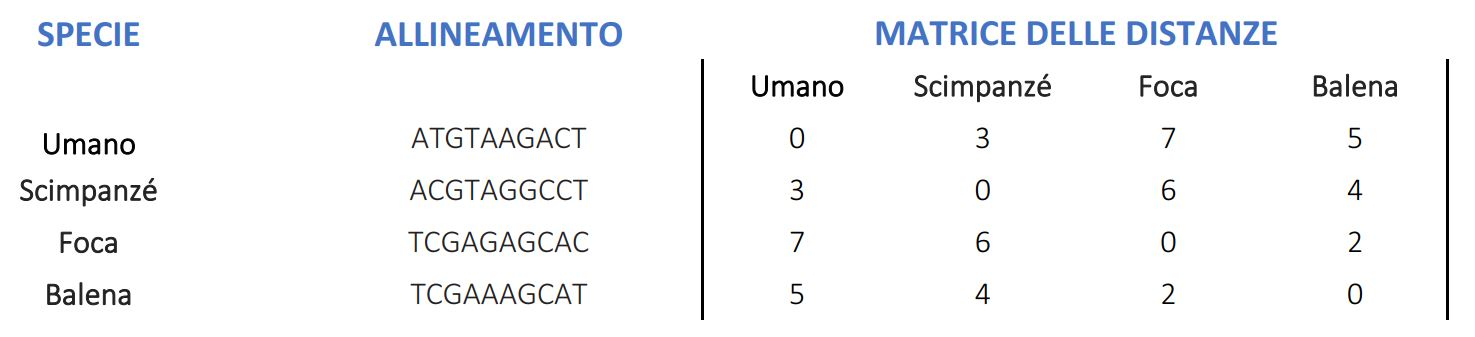
\includegraphics[width=\linewidth]{distance_matrix_example.jpg}
 	\caption{Esempio di matrice delle distanze.}
  	\label{fig:DistanceMatrix}
\end{figure}
\newline
Dalla figura 5 è possibile notare che la sequenza di DNA della foca risulta molto più simile a quella della balena, in quanto la distanza è $2$, piuttosto che con l'umano, la cui distanza invece è $7$.
\newpage

TODO:
\begin{enumerate}
	\item rileggere bene il paragrafo di sopra
	\item elencare le priperità degli alberi  (ad esempio "Si dice che un albero $T$ si \textit{adatta} ad una matrice delle distanze $D$ se per ogni coppia di foglie $i$ e $j$ si ha che $d_i,_j(T)=D_i,_j$." ecc)
	\item cominciare a spiegare gli algoritmi
\end{enumerate}
\begin{center}
\textbf{Problema degli alberi basati sulla distanza:}
\newline
\textit{Dato in \textbf{input} una matrice delle distanze si ottiene in \textbf{output} un albero evolutivo adattato alla matrice stessa.}
\end{center}
Denotando con $d_i,_j(T)$ la distanza evolutiva tra la 
Si dice che un albero $T$ si \textit{adatta} ad una matrice delle distanze $D$ se per ogni coppia di foglie $i$ e $j$ si ha che $d_i,_j(T)=D_i,_j$.